\documentclass[mathserif,fleqn]{beamer}


\usepackage{amsmath}
%\usepackage{amsthm}
\usepackage{amssymb}
\usepackage[justification=justified,font=footnotesize]{caption}
%\usepackage{cancel}
%\usepackage{enumerate}
%\usepackage[stable]{footmisc}
\usepackage{fancyvrb}
\usepackage{graphicx}
%\usepackage{hyperref}
\usepackage[utf8x]{inputenc}
\usepackage{color,listings}
%\usepackage{mathpartir}
%\usepackage{relsize}
%\usepackage{setspace}
%\usepackage{stmaryrd}
%\usepackage{listings}
%\usepackage{placeins}
\usepackage{multicol}
%\usepackage{txfonts}
\usepackage{url}
\usepackage[all]{xy}
%\usepackage{tikz}
%\usetikzlibrary{arrows,shapes,decorations.pathmorphing,backgrounds,positioning,fit,petri}
\usepackage[T1]{fontenc}% optional T1 font encoding
\usepackage{amsmath}
\usepackage{fancyhdr}
%\usepackage{kantlipsum}
%\interdisplaylinepenalty=2500
%\usepackage[cmintegrals]{newtxmath}
\usepackage{eso-pic}


%\usepackage[titles]{tocloft}
%\renewcommand{\cftchapfont}{\bfseries}
%\usepackage[Conny]{fncychap}
%\ChNameVar{\centering\Large\rm\bfseries}
%\ChNumVar{\Large}
%\ChRuleWidth{1pt}
%\ChTitleVar{\centering\Large\rm}

\usepackage{array}
\usepackage{mdwmath}
\usepackage{mdwtab}
\usepackage{eqparbox}

% predefined names
\newcommand{\pvslm}{\textsf{pvslm}}


\hypersetup{pdfstartview={FitH}}
\setbeamertemplate{frametitle}[default][center]
\useinnertheme{rectangles}
%\useoutertheme{infolines}

\definecolor{niceblue}{RGB}{214,214,240}
\definecolor{nicebluefg}{RGB}{51,51,179}

% title page
\setbeamercolor{title}{bg=niceblue}
\setbeamerfont{title}{series=\bfseries}
% frame title
\setbeamercolor{frametitle}{bg=niceblue}
\setbeamerfont{frametitle}{series=\bfseries}
% block title
\setbeamerfont{block title}{series=\bfseries}
\setbeamerfont{section in toc}{series=\bfseries}
% footer
\setbeamertemplate{navigation symbols}{}
% alerted text
\setbeamercolor{alerted text}{fg=nicebluefg}
\setbeamerfont{alerted text}{series=\bfseries}

% custom itemization and enumeration environments
\newenvironment{customitemize}[1][0]
  { \begin{itemize}
    % set spacing between items
    \addtolength{\itemsep}{#1\baselineskip}
    % set spacing between lines
    %\addtolength{\baselineskip}{#1\baselineskip} 
  }
  { \end{itemize} }
\newenvironment{customenumerate}[1][0]
  { \begin{enumerate}
    % set spacing between items
    \addtolength{\itemsep}{#1\baselineskip}
    % set spacing between lines
    %\addtolength{\baselineskip}{#1\baselineskip} 
  }
  { \end{enumerate} }

\newenvironment{outeritemize}
  { \begin{customitemize}[0.5] }
  { \end{customitemize} }
\newenvironment{inneritemize}
  { \begin{customitemize}[0.2] }
  { \end{customitemize} }
  
\newenvironment{outerenumerate}
  { \begin{customenumerate}[0.5] }
  { \end{customenumerate} }
\newenvironment{innerenumerate}
  { \begin{customenumerate}[0.2] }
  { \end{customenumerate} }

\newcommand\Mark[1]{\textsuperscript#1}

\title{ 
  Library Management for PVS
}

\author[M. Romero]{
  {\bf Miguel Romero\Mark{1}} \and Camilo Rocha\Mark{2}
}

\institute[ECI]{
  \large \Mark{1}Escuela Colombiana de Ingenier\'ia Julio Garavito\\ \Mark{2}Pontificia Universidad Javeriana, Cali 
}

\date[MPL 09.27.2016]{
  11CCC\\
  September 29, 2016
}

% PDF settings
\hypersetup{%
  pdftitle=\@title,%
  pdfauthor=\@author%
}	

\begin{document}

\begin{frame}
  \titlepage
\end{frame}

% pending Context
\begin{frame}
  \frametitle{Context}
 
   \begin{outeritemize}
   \item  The Prototype Verification System (PVS) is a verification system comprising a specification language integrated with support tools and a theorem prover
   \item The PVS system has been used in state-of-the-art formal methods projects as a productive environment for constructing and maintaining collections of theories, both in industry and in research.
   \item In \cde{pvslm}, the description language is designed to represent a PVS library as a collection of packages, with a package consisting of a collection of PVS theories. 
   \end{outeritemize}
\end{frame}

% pending Problem
\begin{frame}
  \frametitle{The Problem}
  Given the increasing size of mathematical developments in the form of libraries and the growing need for and adoption of mechanized proof environments, such as PVS, it is important to have tools for managing such libraries.
\end{frame}

% pending Contribution
\begin{frame}
  \frametitle{Main Contribution}
   \begin{outeritemize}
   \item \cde{pvslm} is an utility for assisting in the management of PVS libraries, comprising:
   \begin{inneritemize}
      \item[] a description language for annotating PVS libraries
      \item[] an implementation for managing PVS libraries annotated with this language
    \end{inneritemize}
    \item The \cde{pvslm} implementation is written in the Python programming language and it can manage any (annotated) PVS library that is publicly available from a \cde{pvslm} server through the internet.
   \end{outeritemize}
\end{frame}

% Roadmap
\begin{frame}
  \frametitle{Roadmap}
  \tableofcontents
\end{frame}

% Description Language
\section{Description Language}

\begin{frame}
  \frametitle{Roadmap} 
  \tableofcontents[currentsection]
\end{frame}

\begin{frame}
  \frametitle{Description Language}

The \cde{pvslm} tool distinguishes three levels of aggregation for PVS
sources. A PVS theory is the building block of a library managed by
\cde{pvslm}. A {\em package} is a collection of theories.  A {\em
  library} is at the top level of aggregation, comprising a collection
of packages.

\end{frame}

\begin{frame}
  \frametitle{Description Language: BNF-like notation}
  
    \begin{table}
    \begin{tabular}{r c p{6cm}}
      \hline \\
      $\nterm{\cde{metadata}}$ & ::= & $\nterm{\cde{header}} \; \nterm{\cde{body}}$ \\
      $\nterm{\cde{header}}$ & ::= & `/' $\nterm{\cde{theorylist}}$ \\
      $\nterm{\cde{theorylist}}$ & ::= & $\nterm{\cde{theory}} \mid \nterm{\cde{theory}}$ `,' $\nterm{\cde{theorylist}}$ \\
      $\nterm{\cde{body}}$ & ::= & $(\nterm{\cde{packagedep}} \mid \nterm{\cde{theorydep}})*$ \\
      $\nterm{\cde{packagedep}}$ & ::= & $\nterm{\cde{package}}$ `/' $\nterm{\cde{theorylist}}$ \\
      $\nterm{\cde{theorydep}}$ & ::= & $\nterm{\cde{theory}}$ `:' $\nterm{\cde{qualtheorylist}} ?$ \\
      $\nterm{\cde{qualtheorylist}}$ & ::= & $\nterm{\cde{qualtheory}} \mid \nterm{\cde{qualtheory}}$ `,' $\nterm{\cde{qualtheorylist}}$ \\
      $\nterm{\cde{qualtheory}}$ & ::= & $(\nterm{\cde{package}}\; \text{`@'})?$ $\nterm{\cde{theory}}$ \\
      \\
      \hline
    \end{tabular}
    \caption{Syntax of the \cde{top.dep} metadata file in NASALib.}
  \end{table}
  
\end{frame}

\begin{frame}
  \frametitle{Description Language: Example}
  \begin{figure}
   \centering
   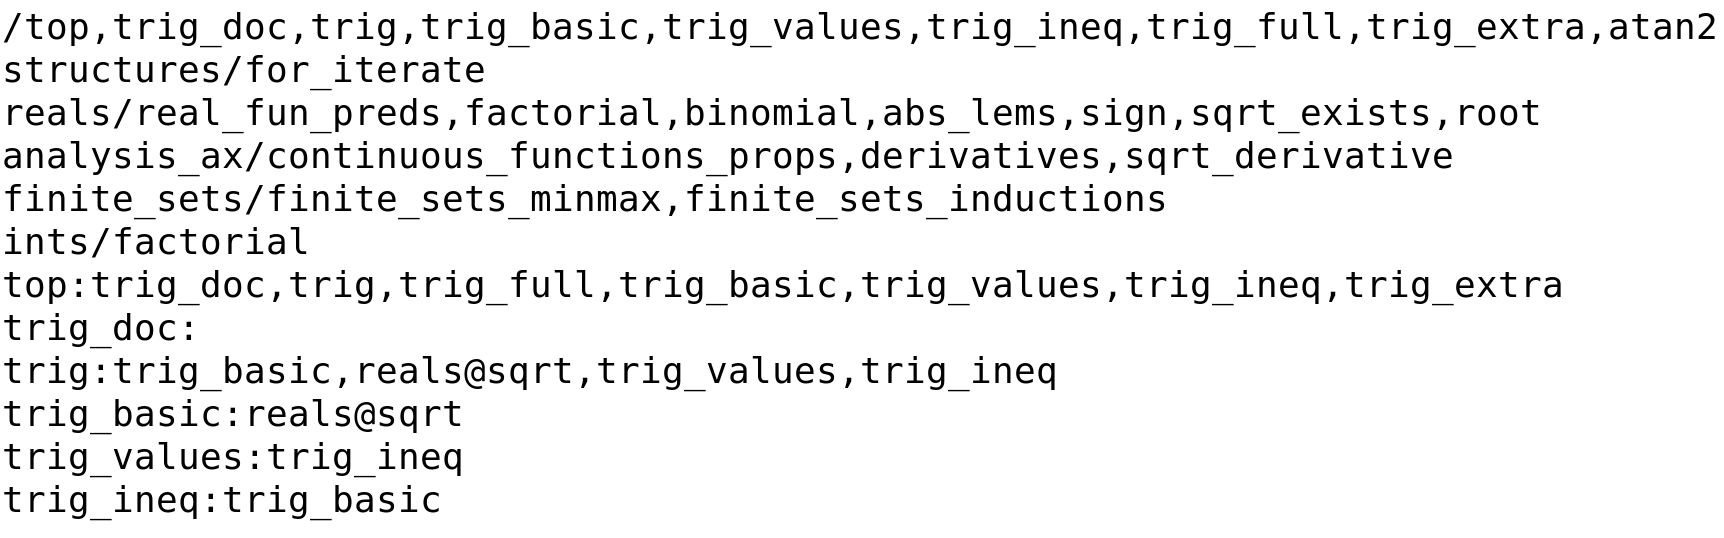
\includegraphics[width=11cm]{top.png}
   \caption{Overview of metadata file for package trig in NASALib.}
  \end{figure}

\end{frame}

% Obtaining the pvslm implementation
\section{Obtaining the \cde{pvslm} Implementation}

\begin{frame}
  \frametitle{Roadmap} 
  \tableofcontents[currentsection]
\end{frame}

\begin{frame}
   \frametitle{How to obtain \cde{pvslm}}

   The \cde{pvslm} tool can be installed automatically from the terminal in
   unix systems by issuing the following command: 
   
   \bigskip
   
   %
   \begin{small}
   \begin{tt}
     curl http://migueleci.github.io/pvslm/downloads/pvslm-conf.py 
      -o pvslm-install $\&\&$ chmod +x pvslm-install $\&\&$ 
      python ./pvslm-install
   \end{tt}
   \end{small}
   %

\end{frame}

% Available Commands
\section{Available Commands}

\begin{frame}
  \frametitle{Roadmap} 
  \tableofcontents[currentsection]
\end{frame}

\begin{frame}
  \frametitle{Available Commands: Libraries}
  
   \begin{outeritemize}
   \item Adding a library source (i.e., command \cde{-a}) with a
    name, a short description, and a \cde{git} URL.
   \item Deleting a library source (i.e., command \cde{-d}) with
    the given name.
   \item Cloning a library source (i.e., command \cde{-c}) with the
    given name.
   \item Updating a library source (i.e., command \cde{-u}) with
    the given name.
   \item Removing the clone of a library source (i.e., command
    \cde{-r}) with the given name.
   \end{outeritemize}
  
\end{frame}

\begin{frame}
  \frametitle{Available Commands: Packages}
  
   \begin{outeritemize}
   \item Installing and updating a given package (i.e., command
    \cde{-i}) from a given library source, including {\em all} its
    dependencies.
  \item Updating a given package (i.e., command \cde{-u}) from a given
    library source, including {\em all} its dependencies.
  \item Deleting a given package (i.e., command \cde{-d}) from a given
    library source (local copy), including all packages that depend on
    it.
  \item Listing the contents (i.e., command \cde{-l}) from a given
    library source.
   \end{outeritemize}
  
\end{frame}

% Conclusion
\section{Conclusion}

\begin{frame}
  \frametitle{Roadmap} 
  \tableofcontents[currentsection]
\end{frame}

\begin{frame}
  \frametitle{Conclusion}

  \begin{outeritemize}
  \item This tool features support for different library sources, libraries with several theories, and dependencies among the theories (within the same library source).
  \item  The tool is freely available for download and it is distributed under GNU's GPLv3 license.
  \item It uses a small footprint language for annotating libraries
  \end{outeritemize}

\end{frame}

\begin{frame}

  \begin{center}
      {\LARGE \tbf{Thank you.}}
  \end{center}
\end{frame}

\end{document}

\begin{frame}
  \frametitle{The Problem}

\end{frame}

